\documentclass{beamer}
\usepackage{beamerthemesplit}
\usepackage[utf8]{inputenc}
\begin{document}
\title{Metriikat ohjelmiston laadun mittaamiseen}
\author{Janne Haapsaari}
\date{\today}

\frame{\titlepage}

\section{Ohjelmisto}
\frame{\frametitle{Ohjelmistot}
  \begin{itemize}
    \item Modernit ohjelmistot ovat monimutkaisia kokonaisuuksia. \pause
    \item Täsmällinen suunnittelu etukäteen vaikeaa. \pause
    \item Ohjelmistoon kohdistuu muutoksia koko sen elinkaaren ajan. 
    \begin{itemize}
      \item Muuttuvat vaatimusmääreet, toimintaympäristö, virheet ohjelmistossa\dots
    \end{itemize}
  \end{itemize}
}

\section{Ohjelmiston laatu} 
\frame{\frametitle{Ohjelmiston laatu}
  \begin{itemize}
    \item IEEE: Ohjelmiston kyky toteuttaa sille asetetut vaatimukset sekä asiakkaan tai käyttäjän sille asettamat vaatimukset ja odotukset.\pause
    \item ISO 9000: Ominaispiirteiden kokonaisuus, jotka vaikuttavat ohjelmiston kykyyn täyttää sille asetettuja tai oletettuja tarpeita. \pause
    \item Pressman: Ohjelmiston kyky noudattaa sille täsmällisesti määriteltyjä toiminnallisuus- ja tehokkuusvaatimuksia, explisiittisesti dokumentoituja käytäntöjä sekä vaatimuksia joita voidaan olettaa löytyvän ammattimaisesta sovelluksesta.
  \end{itemize}
}

\frame{\frametitle{Ohjelmiston laatu}
  \begin{itemize}
    \item Ohjelmiston laadun täsmällinen arviointi on vaikeaa. \pause
    \item Laadun määritelmille yhteistä on asiakas-/käyttäjälähtöisyys.
  \end{itemize}
}

\frame{\frametitle{Ohjelmiston laadun arviointi}
  \begin{itemize}
    \item ISO 25010 standardi esittelee ohjelmiston laatumallin, joka jakaa laadun ulkoisiin ja sisäisiin laatutekijöihin.
  \end{itemize}
}

\frame{\frametitle{Ulkoiset laatutekijät}
  \begin{itemize}
    \item Kuvaavat ohjelmiston toiminnallisuutta ja käyttäjäkokemusta. \pause 
      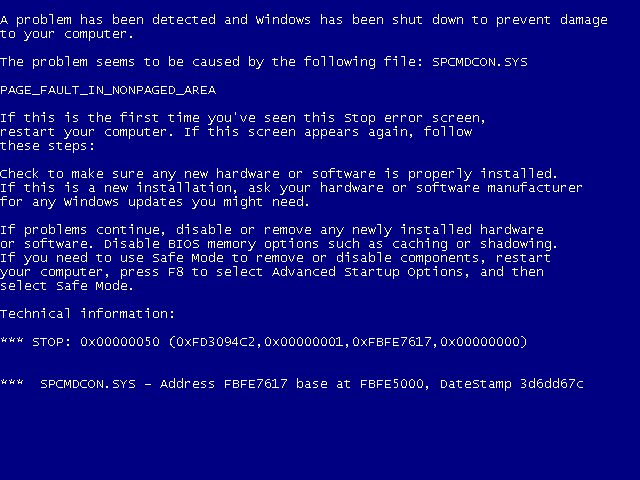
\includegraphics[scale=0.25]{bsod.png}\pause
    % Poistetaanko allaolevat?
    \item Toiminnallinen sopivuus, käytettävyys, luotettavuus, standardinmukaisuus\dots
  \end{itemize}
}

\frame{\frametitle{Sisäiset laatutekijät}
  \begin{itemize}
    \item Kuvaavat ohjelmiston sisäistä toteutusta ja rakennetta. \pause
    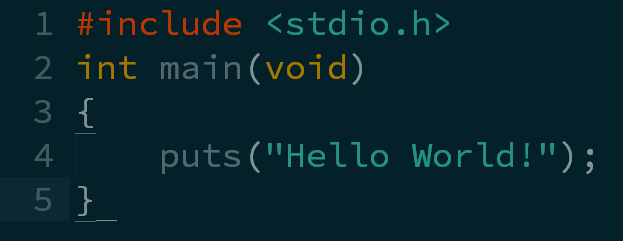
\includegraphics[width=80mm]{hello_world.png} \pause
    % Poistetaanko allaolevat?
    \item Sisäisiä tekijöitä: suorituskyky, turvallisuus, yhteensopivuus, siirrettävyys, ylläpidettävyys\dots
  \end{itemize}
}

\frame{\frametitle{Miksi ohjelmistometriikoita tarvitaan?}
  \begin{itemize}
    \item Jopa 60-80\% ohjelmistoprojekteista ylittää alkuperäisen budjetti- ja aikatauluarviot.\pause
    \item Ohjelmistot laajoja, resurssit rajallisia. Resurssien parempi kohdentaminen.\pause
    \item Mitä aikaisemmin virhe havaitaan, sitä halvempaa sen korjaaminen on.
  \end{itemize}
}

\section{Ohjelmistometriikat}
\frame{\frametitle{Ohjelmistometriikat}
  \begin{itemize}
    \item Ohjelmistometriikoita on tutkittu koko sen ajan kun ohjelmistoja on tuotettu. \pause
    \item Kirjallisuudessa ensimmäiset ohjelmistometriikat esiteltiin 1960-luvulla. \pause
    \item Pyrkivät rajoittamaan ohjelmiston fyysistä kokoa. \pause
    \item Metriikat analysoivat ohjelmistoa ja etsivät siitä virheherkkiä osia.
  \end{itemize}
}

\frame{\frametitle{Perinteiset ohjelmistometriikat}
  \begin{itemize}
    \item Halsteadin menetelmä laski operaattoreiden ja operandien määrää. \pause
    \item McCaben Syklomaattinen kompleksisuus, joka arvioi ohjelmiston monimutkaisuutta kontrollipolkujen määrän avulla. \pause
    \item Chidamberin ja Kemererin oliopohjaiset metriikat.
  \end{itemize}
}

\frame{\frametitle{Modernit ohjelmistometriikat}
  \begin{itemize}
    \item Suhteellinen koodikirnu. \pause
    \item Kokonaisvaltaiset metriikat (Bayes-verkko).\pause
    \item Verkkoanalyysipohjaiset metriikat.\pause
    \item Staattinen koodianalyysi.\pause
    \item Koneoppiminen.
  \end{itemize}
}

\frame{\frametitle{Tutkielmassa käsiteltävät ohjelmistometriikat}
  \begin{itemize}
    \item Oliopohjaiset CK-metriikat.
    \item Suhteellinen koodikirnu.
    \item Kokonaisvaltaiset metriikat (Bayes-verkko)
  \end{itemize}
}

\frame{\frametitle{Oliopohjaiset metriikat}
  \begin{itemize}
    \item Perinteiset ohjelmistometriikat eivät huomioineet olio-ohjelmoinnille tyypillisiä rakenteita. \pause
    \item Olioita, luokkia, periytymistä, olioiden välistä viestittelyä\dots
  \end{itemize}
}

\frame{\frametitle{Oliopohjaiset metriikat}
  \begin{itemize}
    \item Chidamberin ja Kemererin metriikka koostuu kuudesta laatua arvioivasta mittarista. \pause
    \begin{itemize}
      \item Painotettu luokan metodien määrä.
      \item Perimäpuun syvyys.
      \item Välittömien aliluokkien määrä.
      \item Luokkien välinen kytkeytyvyys.
      \item Luokan vaste.
      \item Metodien yhdenmukaisuuden puute.
    \end{itemize} \pause
    \item Voidaan laskea jo ennen toteutusvaihetta.
  \end{itemize}
}

\frame{\frametitle{Suhteellinen koodikirnu}
  \begin{itemize}
    \item Mittaa ohjelmistoon tehtäviä muutoksia ja niiden laajutta tietyllä aikavälillä. \pause
    \item Useasti muuttuva ohjelmiston osa sisältää enemmän virheitä kuin osa joka muuttuu vähemmän. \pause
    \item Mitattavat tiedot kerättävissä helposti versionhallintajärjestelmästä.
  \end{itemize}
}

\frame{\frametitle{Suhteellinen koodikirnu}
  \begin{itemize}
    \item Koodikirnun absoluuttiset mittarit: \pause
      \begin{itemize}
        \item Koodirivien yhteenlaskettu määrä.
        \item Muokattujen koodiriven määrä.
        \item Poistettujen koodirivien määrä.
        \item Tiedostojen määrä.
        \item Muutoksen ajanjakso.
        \item Muutosten määrä.
        \item Muokattujen tiedostojen määrä.
      \end{itemize}
  \end{itemize}
}

\frame{\frametitle{Suhteellinen koodikirnu}
  \begin{itemize}
    \item Absoluuttisten mittareiden arvot ovat sellaisenaan heikompia indikaattoreita ohjelmiston virhetiheydestä. \pause
    \item Sen sijaan absoluuttisten mittareiden väliset suhteelliset arvot toimivat paremmin.
  \end{itemize}
}

\frame{\frametitle{Suhteellinen koodikirnu}
  \begin{itemize}
    \item Koodikirnun suhteelliset mittarit: \pause
      \begin{itemize}
        \item Muokattujen koodirivien määrä / Koodirivien yhteenlaskettu määrä.
        \item Poistettujen koodirivien määrä / Koodirivien yhteenlaskettu määrä.
        \item Muokattujen tiedostojen määrä / Tiedostojen määrä.
        \item Muutosten määrä / Muokattujen tiedostojen määrä.
        \item Muutoksien ajanjakso / Tiedostojen määrä.
        \item Muokattujen ja poistettujen koodirivien määrä / Muutoksien ajanjakso.
        \item Muokattujen koodirivien määrä / Poistettujen koodirivien määrä.
        \item Muokattujen ja poistettujen koodirivien määrä / Muutosten määrä.
      \end{itemize}
  \end{itemize}
}

\frame{\frametitle{Suhteellinen koodikirnu}
  \begin{itemize}
    \item Suhteellisten mittareiden korkea arvo indikoi virheherkkää ohjelmiston osaa. \pause
    \item Suhteellisia arvoja vertaamalla voidaan vähentää yksittäisen kehittäjän tyylin vaikutusta tuloksiin.
  \end{itemize}
}

\frame{\frametitle{Bayes-verkkoon perustuva metriikka}
  \begin{itemize}
    \item Kokonaisvaltainen metriikka, joka rakentuu perinteisten metriikoiden varaan.\pause
    \item Ottaa huomioon epävarmuustekijöitä ja syy-seuraussuhteita. \pause
    \begin{itemize}
      \item Ongelmakentän vaikeus, ohjelmiston käyttökohde, työntekijöiden kokemus\dots
    \end{itemize} \pause
    \item Todennäköisyys malli rakentuu edellisten projektien datan ja asiantuntija-arvion varaan.
  \end{itemize}
}

\frame{\frametitle{Bayes-verkkoon perustuva metriikka}
  \begin{itemize}
    \item Vaiheistaa ohjelmistokehityksen (suunnittelu, toteutus, testaus\dots).\pause
    \item Jokaiselle vaiheelle luodaan oma Bayes-verkko. \pause
    \item Verkon tulos toimii syötteenä seuraavan vaiheen verkolle.
  \end{itemize}
}

\frame{\frametitle{Bayes-verkkoon perustuva metriikka}
  \begin{itemize}
    \item Bayes-verkon luokat:
    \begin{itemize}
      \item Lisätty uusi toiminnallisuus.
      \item Määrittely ja dokumentointi.
      \item Suunnittelu ja kehitys.
      \item Testaus ja refaktorointi.
    \end{itemize}    
  \end{itemize}
}

\frame{\frametitle{Bayes-verkkoon perustuva metriikka}
  \begin{center}
    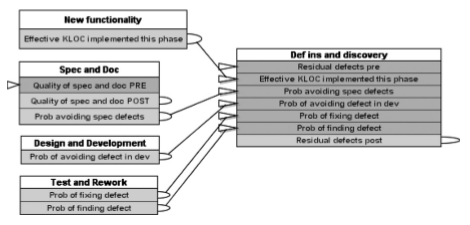
\includegraphics[scale=0.9]{bayes2.png}
  \end{center}
}

\frame{\frametitle{Yleistä ohjelmistometriikoista} 
  \begin{itemize}
    \item Ohjelmistometriikkat on käsitteenä laaja. \pause
    \item Ohjelmistometriikat eivät ole lyöneet läpi ohjelmistoteollisuudessa. \pause
    \item Metriikoiden tehokkuus vaihtelee eri ohjelmointikielten välillä. \pause
    \item Parhaat tulokset saadaan yhdistelemällä metriikoita.
  \end{itemize}
}

\frame{\frametitle{Yleistä ohjelmistometriikoista} 
  \begin{itemize}
    \item Ohjelmistotuotanto on ihmiskeskeistä toimintaa. \pause
    \item Mikään ohjelmistometriikka ei takaa laadukasta ohjelmistoa. \pause
    \item Laadukkaan ohjelmiston toteuttavat ammattitaitoiset tekijät.
  \end{itemize}
}

\section{Kysymyksiä?}
\frame{\frametitle{Kysymyksiä}
  \begin{itemize}
    \item Kiitos!
    \item Kysymyksiä, kommentteja, palautetta?
  \end{itemize}
}
\end{document}
